\section{Results}
\label{sec:results}

% Every number below is taken from the committed exports through the paper index
% (results/vsmt_lean_s3_06_paper_index_154043e.json); sentence-level wording follows EXECUTE LOG-307 A2/A4, LOG-308, LOG-309.

\begin{table*}[t]
\centering
\caption{Test results (single read). Learned arms: mean over five seeds {\tiny$\pm$SD}; rule arms are deterministic. Each column is averaged over the houses its one exclusion list keeps (bottom row). ``--'': not defined (the arm never retracts). $^{(3)}$: only three seeds had a value. Lat.: frames, over recovered objects only; Rec./unrec.: recovered and unrecovered changed (removed, moved or added) objects over all usable episodes. $\downarrow$: lower is better.}
\label{tab:main}
\scriptsize
\setlength{\tabcolsep}{3pt}
% generated by paper/tools/make_tables.py from results/vsmt_lean_s3_05_statistics_8d58475.json and vsmt_lean_s3_06_reanalysis_cd3ee83.json; do not edit by hand

\begin{tabular}{lcccccccccc}
\toprule
 & \multicolumn{2}{c}{Node accuracy} & \multicolumn{1}{c}{Stale} & \multicolumn{2}{c}{False retractions} & \multicolumn{2}{c}{Relocated objects} & \multicolumn{2}{c}{Recovery} & \multicolumn{1}{c}{Contamination} \\
\cmidrule(lr){2-3}\cmidrule(lr){4-4}\cmidrule(lr){5-6}\cmidrule(lr){7-8}\cmidrule(lr){9-10}\cmidrule(lr){11-11}
Arm & F1 & F1$_{\mathrm{IoU}}$ & \textbf{MRR}$\downarrow$ & FRR$_{\mathrm{in}}\!\downarrow$ & FRR$\downarrow$ & \textbf{IdC} & Retr. & Lat.$\downarrow$ & Rec./unrec. & Cont.$\downarrow$ \\
\midrule
\multicolumn{11}{l}{\emph{Simulator instance masks} (87 test houses)} \\
\textbf{VSMT-lean} & 0.853{\tiny$\pm$.004} & 0.490{\tiny$\pm$.002} & 0.115{\tiny$\pm$.020} & 0.192{\tiny$\pm$.032} & 0.221{\tiny$\pm$.036} & 0.211{\tiny$\pm$.050} & 0.254{\tiny$\pm$.049} & 133.6{\tiny$\pm$5.2} & 296/62 & 0.307{\tiny$\pm$.005} \\
\addlinespace[1.5pt]
AssocOnly & 0.851{\tiny$\pm$.004} & 0.488{\tiny$\pm$.000} & 0.642{\tiny$\pm$.034} & -- & -- & 0.104{\tiny$\pm$.013} & 0.108{\tiny$\pm$.014} & 158.3{\tiny$\pm$6.1} & 151/207 & 0.314{\tiny$\pm$.005} \\
NoVersion & 0.854{\tiny$\pm$.005} & 0.490{\tiny$\pm$.002} & 0.102{\tiny$\pm$.024} & 0.163{\tiny$\pm$.021} & 0.185{\tiny$\pm$.023}$^{(3)}$ & 0.006{\tiny$\pm$.005} & 0.141{\tiny$\pm$.023} & 136.4{\tiny$\pm$7.5} & 304/54 & 0.306{\tiny$\pm$.005} \\
HeuristicLabel & 0.632{\tiny$\pm$.000} & 0.401{\tiny$\pm$.001} & 0.192{\tiny$\pm$.004} & 0.897{\tiny$\pm$.002} & 0.926{\tiny$\pm$.001} & 0.134{\tiny$\pm$.000} & 0.174{\tiny$\pm$.004} & 156.2{\tiny$\pm$2.3} & 289/69 & 0.325{\tiny$\pm$.001} \\
HandCost & 0.614 & 0.395 & 0.106 & 0.876 & 0.922 & 0.143 & 0.255 & 127.4 & 316/42 & 0.335 \\
\addlinespace[1.5pt]
TAF & 0.667 & 0.432 & 0.883 & -- & -- & 0.032 & 0.032 & 137.5 & 107/251 & 0.329 \\
ELU-P & 0.660 & 0.422 & 0.075 & 0.924 & 0.967 & 0.006 & 0.188 & 151.3 & 325/33 & 0.330 \\
RAC & 0.640 & 0.416 & 0.093 & 0.797 & 0.916 & 0.000 & 0.228 & 131.1 & 323/35 & 0.320 \\
LOW & 0.763 & 0.462 & 0.654 & -- & -- & 0.000 & 0.026 & 170.0 & 152/206 & 0.368 \\
\addlinespace[1.5pt]
\emph{Houses kept} & 87 & 87 & 62 & 65 & 66 & 58 & 58 & 52 & all & 87 \\
\midrule
\multicolumn{11}{l}{\emph{SAM 2.1 masks} (85 test houses)} \\
\textbf{VSMT-lean} & 0.537{\tiny$\pm$.002} & 0.257{\tiny$\pm$.002} & 0.055{\tiny$\pm$.010} & 0.564{\tiny$\pm$.059} & 0.668{\tiny$\pm$.075} & 0.063{\tiny$\pm$.021} & 0.162{\tiny$\pm$.023} & 124.8{\tiny$\pm$6.2} & 293.6/58.4 & 0.462{\tiny$\pm$.003} \\
\addlinespace[1.5pt]
AssocOnly & 0.528{\tiny$\pm$.003} & 0.255{\tiny$\pm$.001} & 0.235{\tiny$\pm$.013} & -- & -- & 0.082{\tiny$\pm$.019} & 0.107{\tiny$\pm$.022} & 149.2{\tiny$\pm$10.7} & 241.8/110.2 & 0.466{\tiny$\pm$.003} \\
NoVersion & 0.540{\tiny$\pm$.002} & 0.257{\tiny$\pm$.002} & 0.029{\tiny$\pm$.009} & 0.557{\tiny$\pm$.058} & 0.665{\tiny$\pm$.072} & 0.014{\tiny$\pm$.016} & 0.186{\tiny$\pm$.020} & 125.4{\tiny$\pm$5.3} & 301.4/50.6 & 0.462{\tiny$\pm$.003} \\
HeuristicLabel & 0.406{\tiny$\pm$.001} & 0.221{\tiny$\pm$.000} & 0.160{\tiny$\pm$.006} & 0.932{\tiny$\pm$.001} & 0.963{\tiny$\pm$.000} & 0.107{\tiny$\pm$.000} & 0.185{\tiny$\pm$.003} & 136.3{\tiny$\pm$.9} & 283.2/68.8 & 0.397{\tiny$\pm$.000} \\
HandCost & 0.443 & 0.233 & 0.067 & 0.895 & 0.960 & 0.207 & 0.246 & 112.3 & 299/53 & 0.414 \\
\addlinespace[1.5pt]
TAF & 0.456 & 0.246 & 0.745 & -- & -- & 0.042 & 0.054 & 143.0 & 136/216 & 0.401 \\
ELU-P & 0.430 & 0.233 & 0.068 & 0.955 & 0.984 & 0.006 & 0.164 & 137.0 & 311/41 & 0.419 \\
RAC & 0.414 & 0.230 & 0.092 & 0.889 & 0.972 & 0.000 & 0.156 & 123.6 & 305/47 & 0.408 \\
LOW & 0.507 & 0.250 & 0.193 & -- & -- & 0.027 & 0.074 & 110.9 & 209/143 & 0.517 \\
\addlinespace[1.5pt]
\emph{Houses kept} & 85 & 85 & 61 & 71 & 73 & 56 & 56 & 54 & all & 85 \\
\bottomrule
\end{tabular}

\end{table*}

\begin{table*}[t]
\centering
\caption{Primary hypothesis in the pre-registered fixed order, and the original gate (reported, not gating). Adv.: seed-averaged advantage of VSMT-lean (positive favours VSMT-lean; sign flipped for MRR). LB: two-level one-sided 95\% lower bound. Fav.: seeds with a favourable paired difference. 82-1: seed-stability condition. A row holds when LB $>0$ and 82-1 holds; the original gate requires both of its metrics on a front end and is met on neither.}
\label{tab:gate}
\footnotesize
% generated by paper/tools/make_tables.py from results/vsmt_lean_s3_05_statistics_8d58475.json; do not edit by hand

\begin{tabular}{clcccccccc}
\toprule
Step & Front end / metric & VSMT-lean & Control & Adv. & LB & Fav. & 82-1 & Houses & Holds \\
\midrule
\multicolumn{10}{l}{\emph{Primary hypothesis: VSMT-lean vs.\ AssocOnly, fixed testing order}} \\
1 & Inst. / MRR & 0.115 & 0.642 & +0.527 & +0.467 & 5/5 & yes & 62 & \textbf{yes} \\
1 & Inst. / IdC & 0.211 & 0.104 & +0.108 & +0.049 & 5/5 & yes & 58 & \textbf{yes} \\
2 & SAM 2.1 / MRR & 0.055 & 0.235 & +0.180 & +0.135 & 5/5 & yes & 61 & \textbf{yes} \\
3 & SAM 2.1 / IdC & 0.063 & 0.082 & $-$0.020 & $-$0.049 & 1/5 & no & 56 & no \\
\midrule
\multicolumn{10}{l}{\emph{Original gate: VSMT-lean vs.\ the strongest rule-based control per metric (reported, not gating)}} \\
-- & Inst. / MRR vs.\ ELU-P & 0.115 & 0.075 & $-$0.040 & $-$0.081 & 0/5 & no & 62 & no \\
-- & Inst. / IdC vs.\ TAF & 0.211 & 0.032 & +0.180 & +0.124 & 5/5 & yes & 58 & \textbf{yes} \\
-- & SAM 2.1 / MRR vs.\ ELU-P & 0.055 & 0.068 & +0.013 & $-$0.015 & 5/5 & yes & 61 & no \\
-- & SAM 2.1 / IdC vs.\ TAF & 0.063 & 0.042 & +0.021 & $-$0.005 & 4/5 & no & 56 & no \\
\bottomrule
\end{tabular}

\end{table*}

\subsection{Primary hypothesis}
Table~\ref{tab:gate} gives the fixed-order test; intervals for all other comparisons are in Appendix~\ref{app:intervals}.
On ProcTHOR with a simulator instance-segmentation front end, the lifecycle operations learned by this training procedure (fixed training data, recipe and selection; five seeds) leave fewer stale entities and re-attach more relocated objects than the same-recipe association-only ablation: the Missing residual rate falls from 0.642 to 0.115 (two-level one-sided 95\% lower bound of the advantage 0.467) and identity continuity, scored on the same relocated and re-observed objects for every method, rises from 0.104 to 0.211 (lower bound 0.049).
VSMT-lean also met the registered selection constraint (validation MRR 0.176 against \arm{AssocOnly}'s 0.727).
This front end segments almost perfectly; the result concerns memory updates given near-ideal masks.

With SAM~2.1 segmentation the reduction in stale entities holds (0.235 to 0.055; lower bound 0.135), but identity continuity does not improve (0.063 vs.\ 0.082; difference $-0.020$, lower bound $-0.049$, one of five seeds favourable); under the pre-registered fixed testing order the claim does not extend across both segmenters.
This is not because VSMT-lean more often lacked a carrier before the move (35.0 of 132 events against 37.0 for \arm{AssocOnly}, seed means), and among events with a prior carrier it did not re-attach more objects either (conditional column, 35 houses, arm-specific denominators: $-0.027$, 90\% interval $-0.080$ to $+0.021$).
Per house, the SAM~2.1 identity-continuity difference is zero in 39 of 56 houses, favourable in 6 and unfavourable in 11 (Fig.~\ref{fig:per_house}, Appendix~\ref{app:intervals}); the test audit records no per-event causes, so whether the failure arises in recall, association or retraction is not known.
Identity continuity stays low in absolute terms: even with instance masks about four in five relocated objects are not re-attached to their pre-move identity.

\textbf{Node F1.}
Node F1 differs from the association-only ablation by $+0.003$ (90\% interval $-0.003$ to $+0.008$) with instance masks and by $+0.009$ ($+0.005$ to $+0.012$) with SAM~2.1; no non-inferiority margin was registered.
VSMT-lean's large node-F1 lead over the rule-based arms is present in \arm{AssocOnly} as well; it comes with the learned association trained on instance-truth labels, not with the lifecycle operations.

\textbf{Retrieval and recovery against \arm{AssocOnly}} (descriptive, computed after the test).
Retrieval success is higher by $+0.145$ ($+0.087$ to $+0.207$) with instance masks and $+0.055$ ($+0.007$ to $+0.106$) with SAM~2.1, but remains low (0.254 and 0.162) and is an evaluator-built query, not a task result.
VSMT-lean recovers many more changed (removed, moved or added) objects (296 against 151 of 359 with instance masks; 293.6 against 241.8 of 353 with SAM~2.1) and, over the objects each arm recovers, takes fewer frames ($+24.7$, $+4.6$ to $+47.5$; $+24.4$, $+12.4$ to $+38.1$); the two latency means are over different objects.

\subsection{Reversibility: retraction versus deletion}
Replacing retraction by physical deletion with the same cost heads (\arm{NoVersion}, which selected $\tau_r=0.9$ versus 0.8 with instance masks and the same 0.25 with SAM~2.1) gives a slightly higher node F1 (by 0.001 and 0.003; both intervals exclude zero, the instance-mask one narrowly, $-0.0016$ to $-0.0002$) and a lower Missing residual rate (0.102 vs.\ 0.115; 0.029 vs.\ 0.055), but drops identity continuity to 0.006 (instance) and 0.014 (SAM~2.1); with SAM~2.1 \arm{NoVersion} has the highest node F1 (0.540) and lowest MRR (0.029) of all nine arms.
Re-attachment depends on keeping the versions of retracted entities, at a small cost in stale entities, which were fewer for \arm{NoVersion} in all five seeds on both front ends (descriptive ablation, not corrected for multiplicity).
This suggests that, in this learned policy and with this deletion switch, identities are kept mainly along the path ``retract, then reactivate the same identity'', while fewer stale entities come from retraction itself and do not need the kept versions; the test audit does not record the path per event.
With instance masks VSMT-lean's retrieval is also higher than \arm{NoVersion}'s ($+0.113$, $+0.053$ to $+0.174$); with SAM~2.1 it is not ($-0.024$).

\subsection{Source of supervision and learned costs}
With the same network and recipe, hindsight labels from private instance truth give better values than labels copied from \arm{ELU-P}'s decisions (\arm{HeuristicLabel}) on every metric with instance masks (descriptive); with SAM~2.1 they give better node F1, MRR and false-retract rates, but not identity continuity ($-0.044$), retrieval ($-0.023$) or contamination ($-0.065$, \arm{HeuristicLabel} better), and the latency difference ($+11.5$, $-4.5$ to $+27.3$) is not established (Table~\ref{tab:ablations}, Appendix~\ref{app:intervals}).
The node-F1 part probably reflects mostly the association labels, which in \arm{HeuristicLabel} also come from a rule; we did not separate association from existence labels.
Against hand-written costs in the same solver and vocabulary (\arm{HandCost}), learned costs mainly buy more accurate nodes ($+0.240$ and $+0.094$ F1) and far fewer false retractions; MRR is not separated ($-0.009$ and $+0.012$, intervals including zero).
With SAM~2.1 \arm{HandCost} re-attaches and retrieves more relocated objects than VSMT-lean (identity continuity 0.207 vs.\ 0.063; retrieval 0.246 vs.\ 0.162), with node F1 0.443 and false-retract rate 0.960; its association uses only the descriptor cosine, while the learned head also sees distances and box overlap, and whether this helps far-moved objects re-attach is an untested hypothesis.
Because \arm{AssocOnly}'s association is trained with the same private labels, the gain over \arm{AssocOnly} is not evidence for hindsight supervision as such; the source of supervision is what \arm{HeuristicLabel} varies, and there the two front ends disagree.

\subsection{Rule-based arms: trade-offs, not dominance}
\label{sec:rules}

\begin{figure*}[t]
\centering
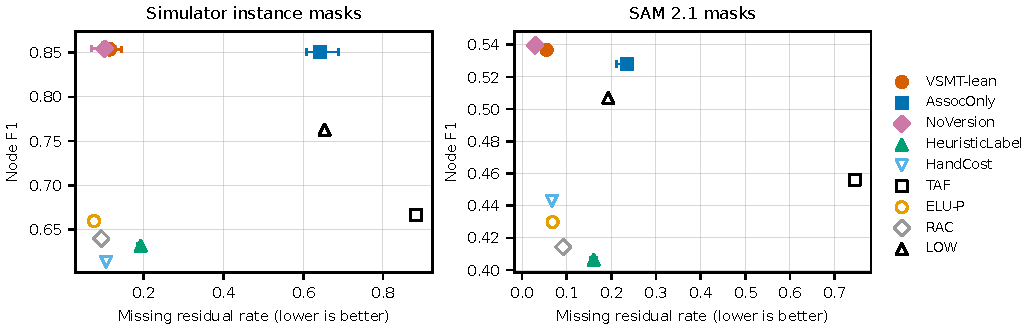
\includegraphics[width=0.9\linewidth]{figures/tradeoff}
\caption{Stale entities against node accuracy on test. Learned arms (filled) with the range over five seeds; rule-based arms and \arm{HandCost} (open) are deterministic. With instance masks no arm is best on both axes; with SAM~2.1 masks the deletion ablation \arm{NoVersion} is best on both axes but keeps almost no identities (identity continuity 0.014, Table~\ref{tab:main}).}
\label{fig:tradeoff}
\end{figure*}

No method dominates on every metric (Table~\ref{tab:main}, Fig.~\ref{fig:tradeoff}; intervals in Table~\ref{tab:rules}, Appendix~\ref{app:intervals}).
The originally registered gate against the strongest rule-based control is not met on either front end: with instance masks \arm{ELU-P} leaves fewer stale entities (0.075 vs.\ 0.115), while 92.4\% of the in-scope entities it retracts (96.7\% overall) belong to objects that are still in place and its node F1 is 0.660 (VSMT-lean 0.853); with SAM~2.1 VSMT-lean has the lower Missing residual rate (0.055 vs.\ 0.068), but the advantage is not established.
\arm{ELU-P} selected the end of its registered grid in three parameters on both front ends; a wider grid might lower its MRR further, and we did not widen it after the test.
VSMT-lean retracts one to two orders of magnitude less often than the retracting rule arms (with instance masks 272 judged retractions per run on the 66 houses of the false-retract list, a seed mean, against 9,492 for \arm{RAC} and 20,901 for \arm{ELU-P}).
Its in-scope false-retract rate (0.192 with instance masks, 0.564 with SAM~2.1; 0.221 and 0.668 overall) is far below that of the rule-based arms that retract and of the \arm{HandCost} and \arm{HeuristicLabel} ablations (0.80--0.96 in scope) and, with instance masks, above \arm{NoVersion}'s (0.163); with SAM~2.1 more than half of the in-scope entities it retracts belong to objects that remained in place.
Retracting a redundant part entity of an over-segmented object also counts as false, since identity is the majority object; the exports do not separate the two cases.
Identity continuity is higher than for every rule arm with instance masks (lower bounds $\geq +0.124$); with SAM~2.1 it is higher than \arm{ELU-P} and \arm{RAC}, not separated from \arm{TAF} and \arm{LOW}, and below \arm{HandCost}.
Retrieval is higher than for \arm{TAF} and \arm{LOW}, but its advantage over the retracting arms is not established (with SAM~2.1 it is below \arm{HandCost}).
Contamination AUC is lower than for every rule arm with instance masks, but with SAM~2.1 VSMT-lean, \arm{NoVersion} and \arm{AssocOnly} (0.462--0.466) are above \arm{TAF}, \arm{ELU-P}, \arm{RAC}, \arm{HandCost} and \arm{HeuristicLabel} (0.397--0.419) and below \arm{LOW} only (0.517); we did not investigate why, and this metric judges staleness by centroid distance only.
VSMT-lean's secondary node column (F1$_\mathrm{IoU}$: 0.490 with instance masks, 0.257 with SAM~2.1) uses Dyn-THOR's matching and overlap rule on different data and is not comparable with numbers in~\cite{dsg2026}.

\subsection{Where the errors are}
Every decision of every run falls into exactly one ledger class (Appendix~\ref{app:ledger}); VSMT-lean and \arm{AssocOnly} miss the correct candidate in recall about equally often in absolute terms (19,885 and 19,242 per run with instance masks).
With SAM~2.1 the share of ambiguous labels about doubles (12.7\% vs.\ 6.8\% for VSMT-lean), suggesting that part of the difficulty lies in the labels; about 10\% of its SAM~2.1 decisions are duplicate fragments.
Arms make different decisions (\arm{AssocOnly} only association decisions), so shares are not ranked across arms, and the ledger does not attribute the gate results to error classes.

\subsection{External check on 3RScan}
\label{sec:external}

\begin{table*}[t]
\centering
\caption{3RScan validation, instance masks rendered from the annotated meshes (proxy truth), every configuration frozen (no retraining or selection). Means over the scenes each metric's list keeps; last rows: advantage of VSMT-lean over \arm{AssocOnly} with the two-level 90\% interval ($^{\ast}$: seed-stability condition holds; this does not imply that the interval excludes zero). Descriptive; not part of the primary hypothesis.}
\label{tab:external}
\scriptsize
\setlength{\tabcolsep}{3pt}
% generated by paper/tools/make_tables.py from results/vsmt_lean_s3_07_statistics_aa94373.json; do not edit by hand

\begin{tabular}{lccccccccc}
\toprule
Arm & F1 & F1$_{\mathrm{IoU}}$ & MRR$\downarrow$ & FRR$\downarrow$ & FRR$_{\mathrm{in}}\!\downarrow$ & IdC & Retr. & Lat.$\downarrow$ & Cont.$\downarrow$ \\
\midrule
\textbf{VSMT-lean} & 0.582{\tiny$\pm$.008} & 0.162{\tiny$\pm$.001} & 0.111{\tiny$\pm$.021} & 0.412{\tiny$\pm$.031} & 0.369{\tiny$\pm$.030} & 0.438{\tiny$\pm$.046} & 0.425{\tiny$\pm$.025} & 24.0{\tiny$\pm$5.9} & 0.531{\tiny$\pm$.005} \\
AssocOnly & 0.543{\tiny$\pm$.018} & 0.161{\tiny$\pm$.002} & 0.137{\tiny$\pm$.039} & -- & -- & 0.338{\tiny$\pm$.089} & 0.351{\tiny$\pm$.086} & 25.4{\tiny$\pm$4.9} & 0.561{\tiny$\pm$.010} \\
NoVersion & 0.583{\tiny$\pm$.009} & 0.162{\tiny$\pm$.001} & 0.118{\tiny$\pm$.025} & 0.408{\tiny$\pm$.040} & 0.369{\tiny$\pm$.010} & 0.351{\tiny$\pm$.074} & 0.407{\tiny$\pm$.050} & 24.6{\tiny$\pm$6.5} & 0.530{\tiny$\pm$.006} \\
HeuristicLabel & 0.437{\tiny$\pm$.001} & 0.151{\tiny$\pm$.000} & 0.599{\tiny$\pm$.017} & 0.744{\tiny$\pm$.002} & 0.664{\tiny$\pm$.002} & 0.390{\tiny$\pm$.007} & 0.411{\tiny$\pm$.041} & 26.3{\tiny$\pm$2.6} & 0.398{\tiny$\pm$.001} \\
HandCost & 0.443 & 0.153 & 0.480 & 0.773 & 0.701 & 0.402 & 0.378 & 19.2 & 0.404 \\
TAF & 0.470 & 0.159 & 0.686 & -- & -- & 0.167 & 0.159 & 24.0 & 0.416 \\
ELU-P & 0.438 & 0.154 & 0.594 & 0.779 & 0.703 & 0.061 & 0.159 & 33.8 & 0.397 \\
RAC & 0.436 & 0.153 & 0.460 & 0.725 & 0.635 & 0.061 & 0.186 & 17.1 & 0.397 \\
LOW & 0.591 & 0.170 & 0.623 & -- & -- & 0.000 & 0.113 & 17.7 & 0.436 \\
\emph{Scenes kept} & 46 & 46 & 38 & 15 & 14 & 11 & 11 & 32 & 46 \\
\midrule
\emph{Adv.\ vs.\ AssocOnly} & +0.039$^{\ast}$ & +0.001 & +0.026 & -- & -- & +0.100$^{\ast}$ & +0.074 & +1.5 & +0.030$^{\ast}$ \\
\emph{\quad 90\% interval} & {\tiny[+0.022, +0.056]} & {\tiny[$-$0.003, +0.006]} & {\tiny[$-$0.031, +0.081]} &  &  & {\tiny[$-$0.004, +0.221]} & {\tiny[$-$0.044, +0.205]} & {\tiny[$-$7.4, +9.9]} & {\tiny[+0.021, +0.038]} \\
\bottomrule
\end{tabular}

\end{table*}

We paired reference scans and rescans of the 3RScan validation split~\cite{rio2019} into 108 usable episodes in 46 scenes; the window between scans has no frames, and poses and alignment come from offline reconstruction.
On these scenes, with instance masks rendered from the annotated meshes (proxy truth) and every configuration frozen, VSMT-lean has a higher node F1 than the association-only ablation ($+0.039$, 90\% interval $+0.022$ to $+0.056$) and leaves fewer stale entities, fewer false retractions and fewer lost identities than the rule-based arms; its advantages over the association-only ablation in Missing residual rate ($+0.026$, $-0.031$ to $+0.081$) and identity continuity ($+0.100$, $-0.004$ to $+0.221$; 11 scenes) are not established, and its contamination AUC is higher than that of every non-learned arm (Table~\ref{tab:external}).
Counter to ProcTHOR, \arm{LOW} has the highest node F1 (0.591; VSMT-lean $-0.009$, $-0.035$ to $+0.017$), \arm{AssocOnly}'s MRR is low (0.137 against 0.642 on ProcTHOR) and the rule arms' are high (0.46--0.69); we did not investigate why.
The SAM~2.1 column could not be computed with the frozen front end (3 of 110 episodes usable).
This check does not show that the primary result reproduces on real data, nor how a learned segmenter or a real robot would fare.

\textbf{Zero-training LLM operator.}
A frozen LLM choosing the same operations from the same sealed feature tables is reported in Appendix~\ref{app:llm}; it is not in the main table and no claim depends on it.
